\FloatBarrier
\subsection{Question 5}
We implement the open-loop system. To close the loop, we apply a moving average controller using \autoref{code:sstr51}. As shown in \autoref{fig:sstr51}, the system remains stable and, when actuated, returns to its equilibrium point at $0$. As shown in \autoref{fig:sstr52}, cummulative loss of the system is bounded.

\begin{code}
	\begin{matlabcode}{firstnumber = 1}
run('SSTR_0.m');

%%  Solve Diophantine equation for d = 2 
d = 2;  % d0=1
[F, G] = diophantine(A, C, d);

%%  Define the MA controller 
MA_controller = tf(conv(F,A), 1, Ts);

%%  Define the open loop system
G_ol = minreal(G_discrete * MA_controller);

%%  Closed-loop system
G_cl = feedback(G_ol, 1);
	\end{matlabcode}
	\captionof{listing}{Moving average controller}
	\label{code:sstr51}
\end{code}

\begin{figure}
	\centering
	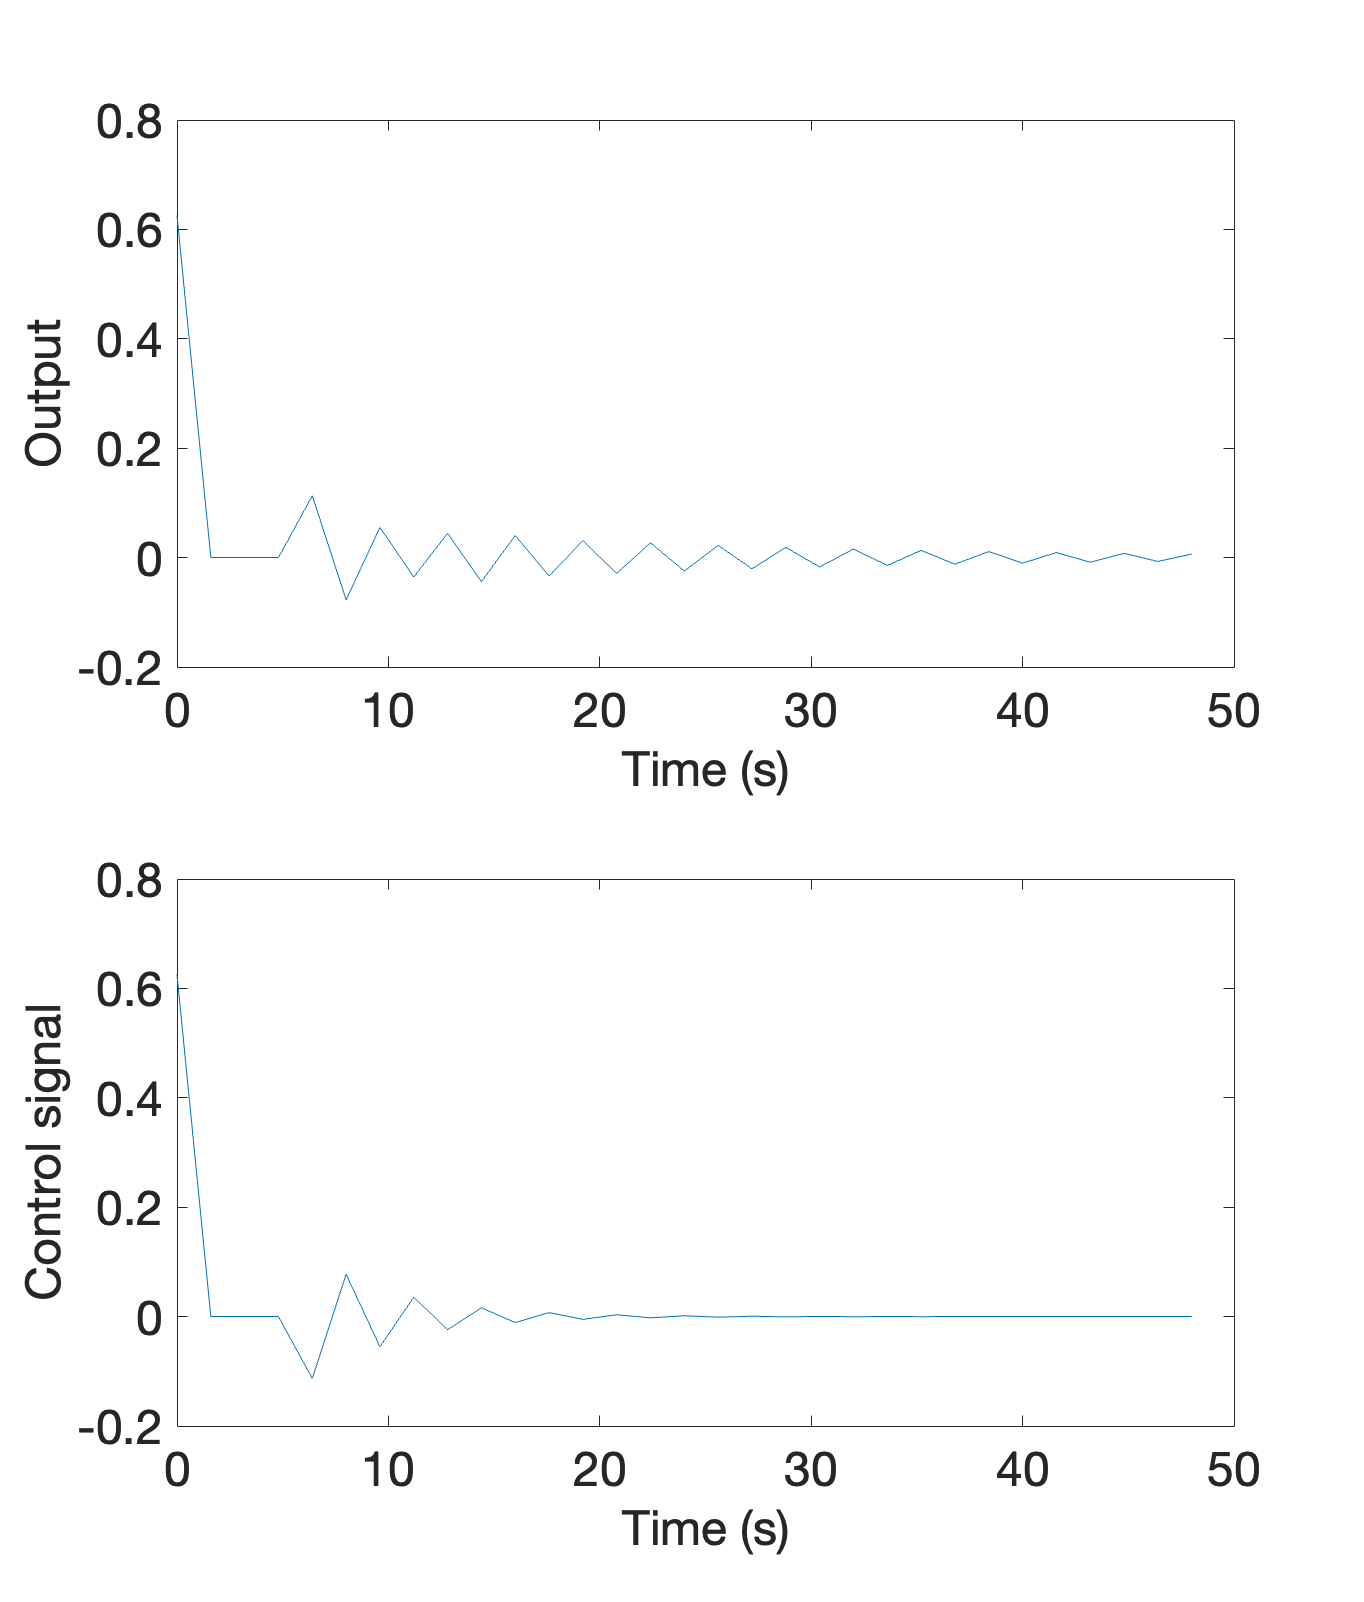
\includegraphics[width=\textwidth]{images/sstr51.png}
	\caption{Output and control of moving average controller}
	\label{fig:sstr51}
\end{figure}

\begin{figure}
	\centering
	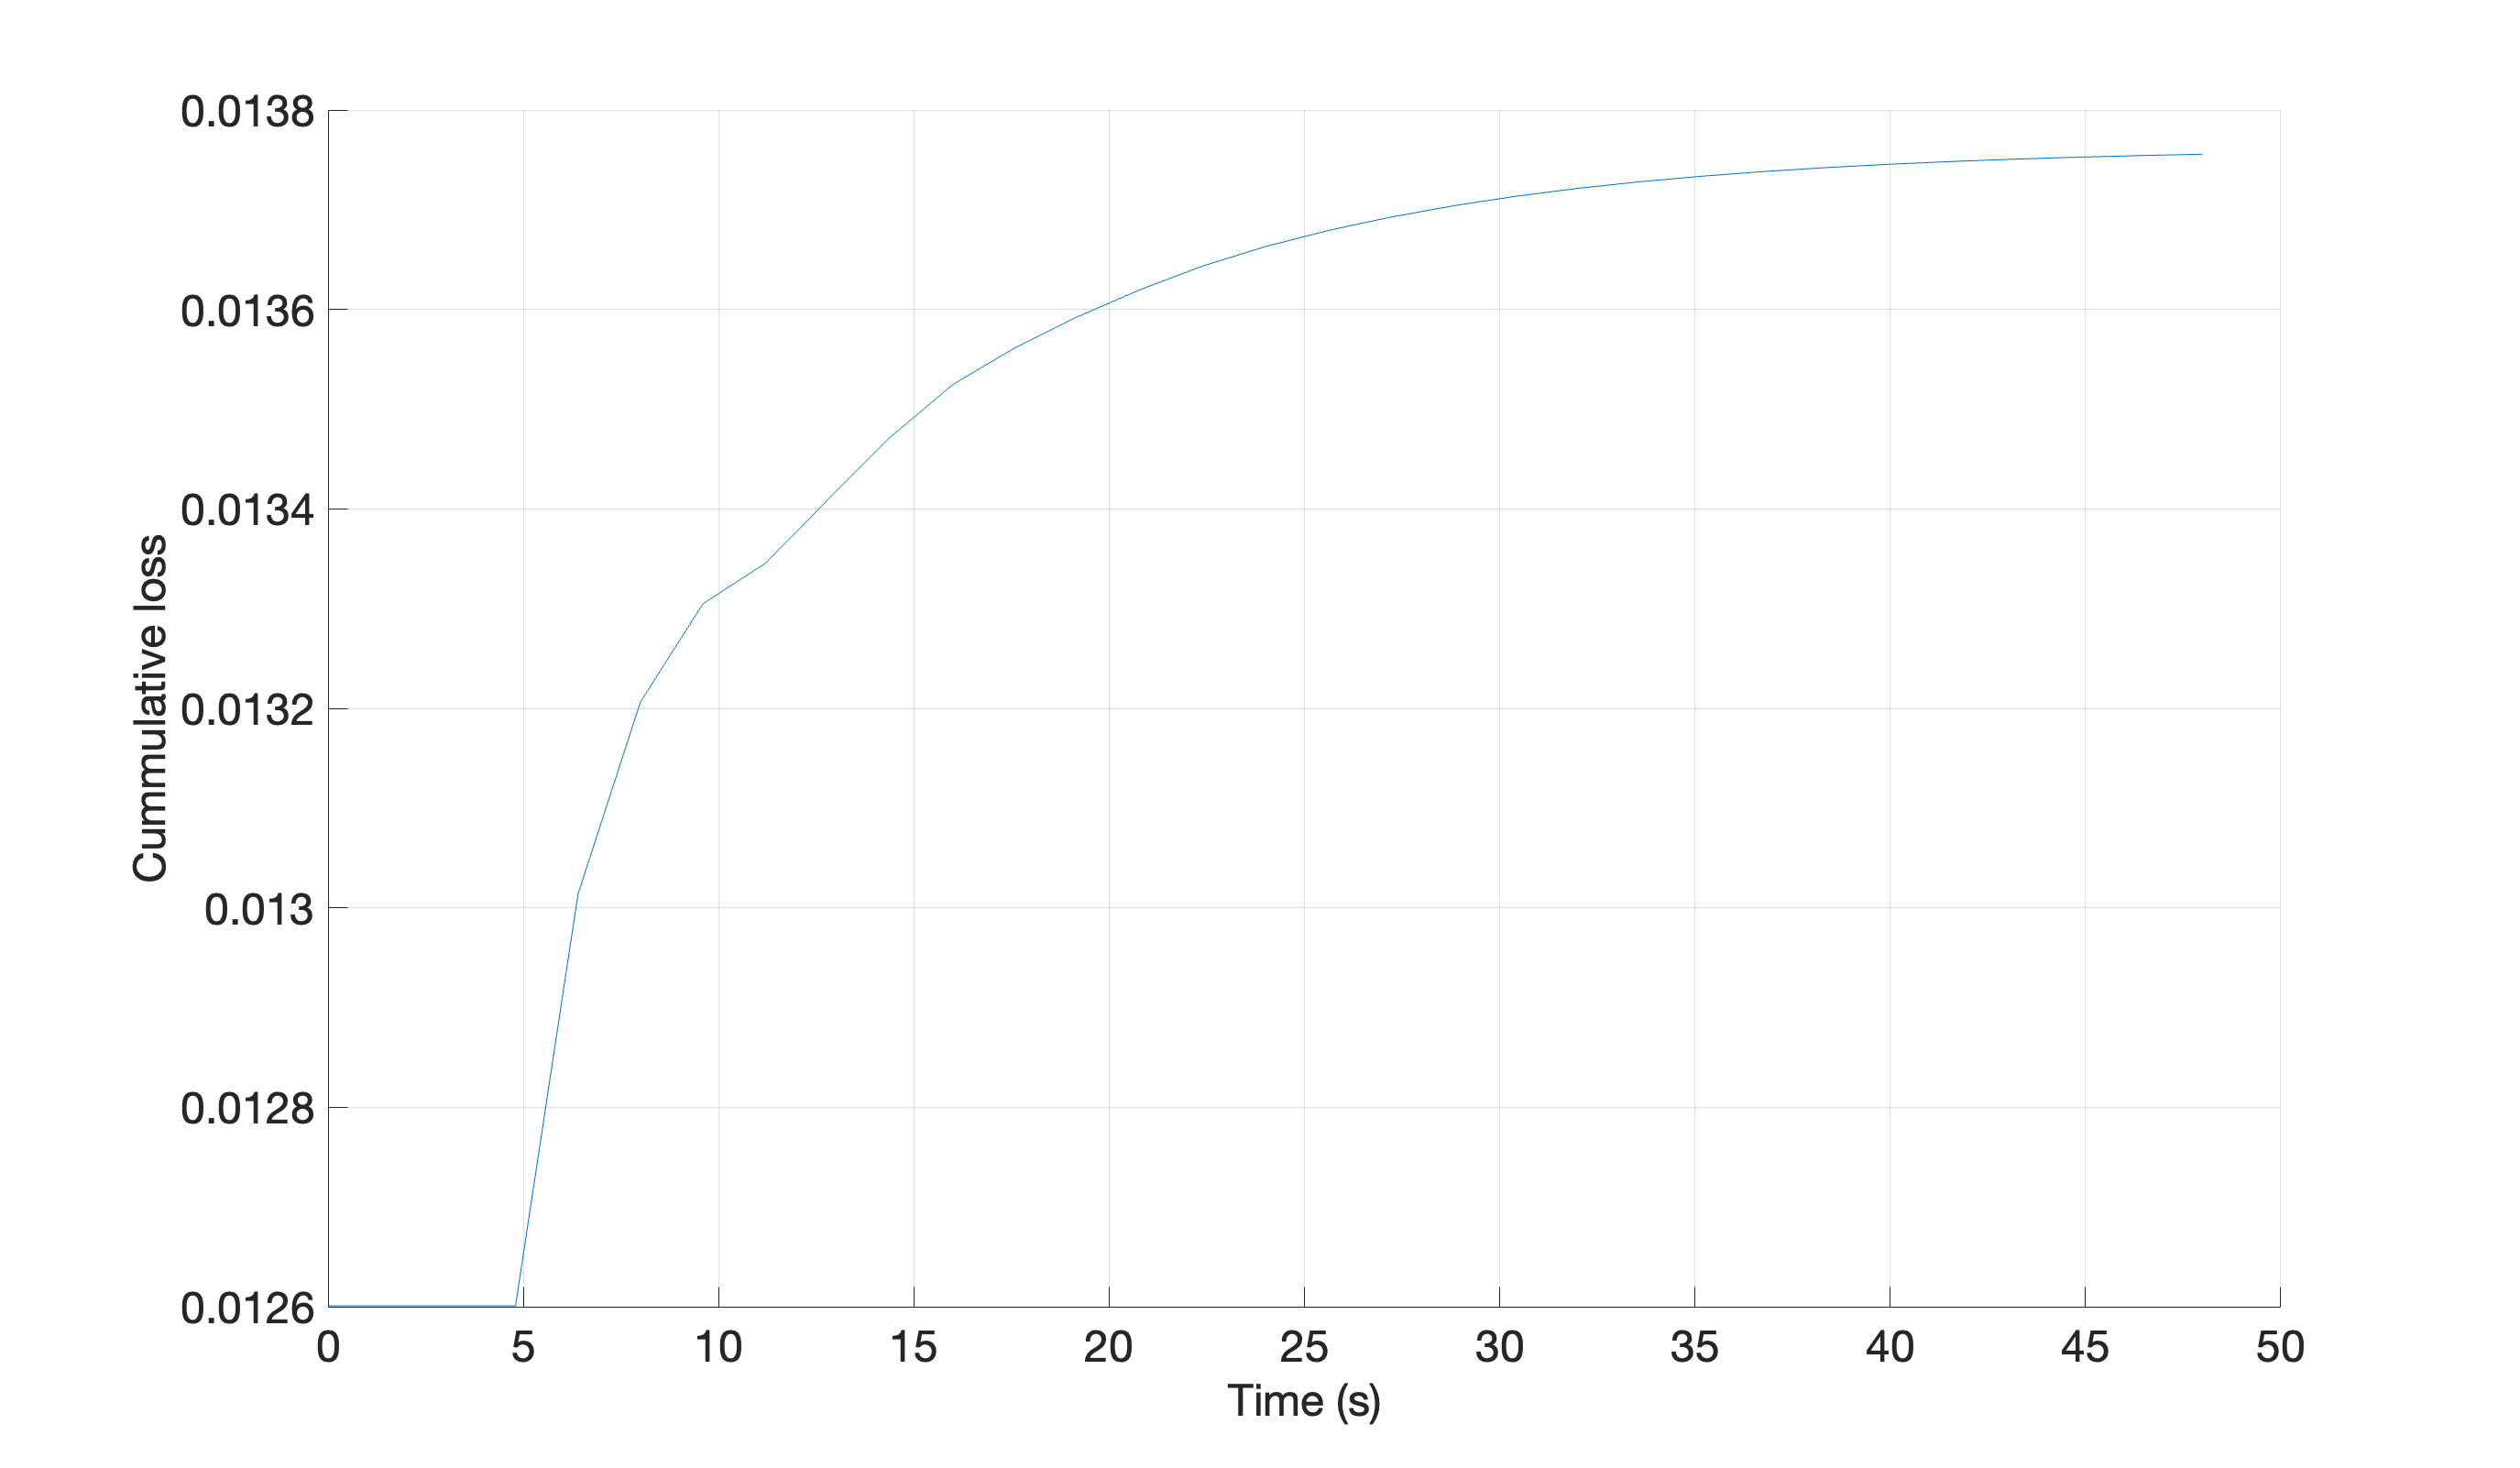
\includegraphics[width=\textwidth]{images/sstr52.png}
	\caption{Cummulative loss of moving average controller}
	\label{fig:sstr52}
\end{figure}

\noindent The code for this section is available at \lstinline|assignment3/SSTR/SSTR_5.m|. 
